\chapter{Verification of models in LAMMPS}
In this chapter, i verify that my LAMMPS setup reproduces known results from the literature. This is necessary to trust the model to go further with modifications.

I use potentials that are already parts of the LAMMPS distribution, so I only need to test that I use LAMMPS correctly. 

\section{TIP4P/ICE}
I want to check that the TIP4P/ICE water potential in LAMMPS reproduces known thermodynamic properties from the literature. The TIP4P potential that comes with lammps, really just handles the massless charged site; the rest of the implementation, namely the rigid bonds and angle, are implemented by the user. Additionally, parameters have to be set. If thermodynamic properties are reproduces, I can be confident that my configuration of the TIP4P potential in LAMMPS is really the potential introduced by \cite{Abascal2005}. 

\subsection{Density of bulk water}
As a quick check of my TIP4P/ICE setup, I want to check the density of bulk water in an NPT simualtion. This property is easily measured, as long as the simulation time is sufficient to gather enough statistics. 

\begin{table}
\centering
\caption{Liquid densities at melting points and melting points for several rigid water models at $P = \text{\SI{1}{\bar}}$. Adapted from \cite{Abascal2005}}
\begin{tabular}{c|cc}
Model & Melting point [K] & Density [\si{\gram\per\cubic\cm}] \\
\hline
TIP4P/ICE 	& 272.2 	& 0.985 \\
TIP4P 		& 232.0 	& 1.002 \\
TIP4P/Ew 	& 245.5 	& 0.992 \\
SPC/E 		& 215.0 	& 1.011 \\
Expt. 		& 273.15 	& 0.999
\end{tabular}
\end{table}

After a few trial simulations, it turns out that the density of water is not a very good way to check whether the implementation is correct, since the values are very similar between the different water models. I have a hard time estimating the density with sufficient confidence to separate it from the density of another water model subjected to the same conditions. Therefore, I go on to investigating more sensitive properties of the water model.

\subsection{Diffusivity and shear viscosity}
It is well established that the relative values of viscosity and diffusivity vary greatly between different water models, eg. \cite{Gonzalez2010,Tazi2012}. That makes these quantities well suited for model verification. To find the shear viscosity $\eta$, I apply equation \ref{eq:GK_shear_viscosity}. Since i do not have access to infinite time series, i plot $\eta(t)$, and use the value it takes when it stabilizes as my estimate. To check that my LAMMPS implementation is correct, I use TIP4P/2005 parameters.  Figure \ref{fig:shear_viscosity_tip4p/2005} shows the estimated shear viscosity from several NVT simulations of \SI{2}{\nano\second} with a density of $\rho = \text{\SI{0.98}{\gram\per\cubic\cm}}$ and temperature $T=\text{\SI{300}{\kelvin}}$. $\eta$ is estimated at \SI{8}{\pico\second} where the variation between the simulations is significantly larger than the fluctuations in the mean. Reference values for shear stress and diffusivity are $\eta = \text{\SI{0.83 \pm 0.05}{\milli\pascal\second}}$ and $D_0 = \text{\SI{2.49 \pm 0.06d-9}{\metre\squared\per\second}}$ from \cite{Tazi2012}.

\begin{figure}
\centering
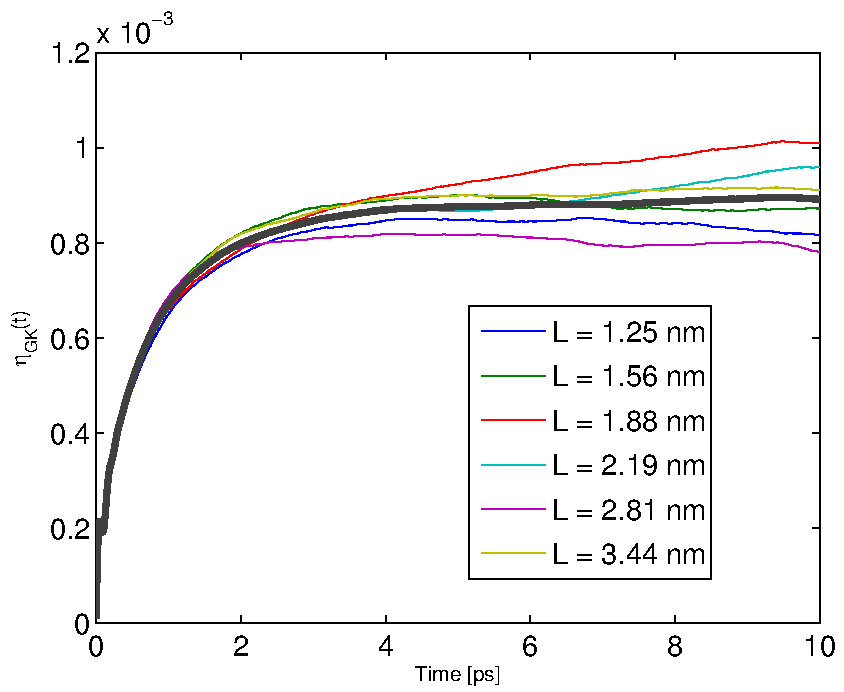
\includegraphics[width=10cm]{../figures/thesis/viscosity_green_kubo_tip4p_2005.pdf}
\caption{Shear viscosity for TIP4P/2005 at \SI{300}{\kelvin} and $\rho = \text{\SI{0.98}{\gram\per\cubic\cm}}$. The viscosity is estimated to $\eta_{GK} = \text{\SI{0.89\pm0.03}{\milli\pascal\second}}$}
\label{fig:shear_viscosity_tip4p/2005}
\end{figure}

In principle, the same simulation can be used to calculate the diffusivity, using the einstein relation \ref{eq:Einstein_diffusivity}. But long simulations are not the way to go when estimating diffusion. An average over several shorter simulations, around \SI{300}{\pico\second}, gives better estimates. 
In Figure \ref{fig:diffusivity_tip4p_2005} I use a weighted linear regression on the diffusion coefficient for different system lengths. As mentioned in the theory section, the diffusion coefficient in a periodic molecular dynamics system depend on the box size, and this finite size effect on it goes like $L^{-1}$. Underlying each (red) data point in Figure \ref{fig:diffusivity_tip4p_2005} are $N_s(L)=9$ simulations of \SI{320}{\femto\second}. Each of these simulations contribute an estimate of the diffusion coefficient using the Einstein relation on the mean squared displacement, and the mean of these $N_s(L)$ estimates is plotted. Error bars are estimated using the standard deviation of the $N_s(L)$ estimates: 
\begin{equation}
	e(L) = \sqrt{\frac{\text{var}(D(L))}{N_s(L)}}
\end{equation}
The expectation vaule of this error should go like $e \propto L^{-3/2}$ (inverse of the square root of the number of particles), which could have been another way to determine the weights.
Then, the regression line is found with weighted linear regression where the weights are:
\begin{equation}
	w(L) = \frac{1}{e(L)^2}
\end{equation}

Using this procedure, I estimate the diffusivity in the TIP4P/2005 model at $T=\SI{300}{\kelvin}$ and $\rho = \SI{0.98}{\gram\per\centi\meter\cubed}$ to $D_0=\text{\SI{2.46\pm0.07d-9}{\meter\squared\per\second}}$, which agrees well with the reference value. For completeness, Figure \ref{fig:msq_tip4p_2005} contains the data underlying the diffusion coefficient calculations. It is included to show how noisy the data are -- the model verification would not be satisfactory with just one simulation for each length of the simulation box.

\begin{figure}
\centering
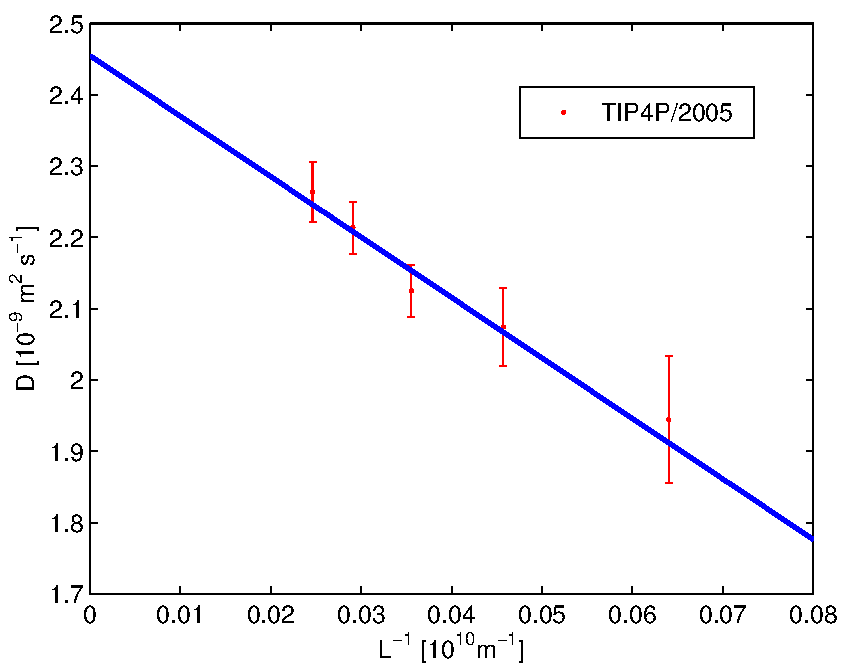
\includegraphics[width=10cm]{../figures/thesis/diffusion_coefficient_tip4p_2005.pdf}
\caption{Diffusivity for TIP4P/2005 for simulations with the same conditions as in Figure \ref{fig:shear_viscosity_tip4p/2005}. The diffusivity is estimated to $D_0=\text{\SI{2.46\pm0.07d-9}{\meter\squared\per\second}}$.}
\label{fig:diffusivity_tip4p_2005}
\end{figure}

\begin{figure}
\centering
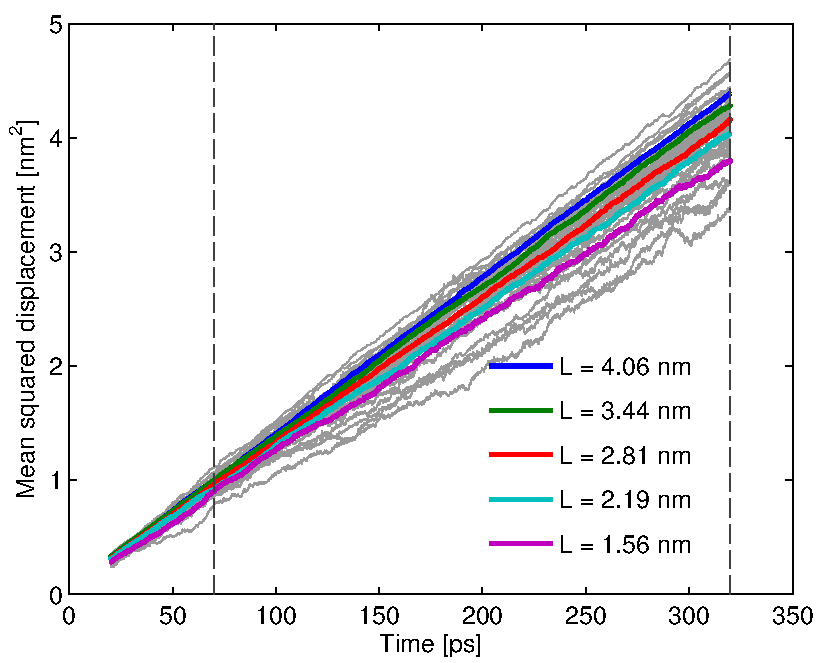
\includegraphics[width=10cm]{../figures/thesis/msq_tip4p_2005.pdf}
\caption{The data underlying Figure \ref{fig:diffusivity_tip4p_2005} (grey, thin lines) and the mean squared displacement averaged over $N_s$ simulation for each system length $L$ (colored, thick lines). Dashed vertical lines indicate the timeframe over which the diffusion coefficient was estimated.}
\label{fig:msq_tip4p_2005}
\end{figure}

Having measured both the shear viscosity and the diffusivity well within the uncertainty of reference values, I trust that my input files for the water model are correct, and go on to checking the methane model.

\section{United atom methane}
Since the methane model is very simple, and only

\section{Stabilizing methane hydrates}
The TIP4P/ICE potential should be able to stabilize a methane hydrate stucture. Therefore, I prepared an S1 hydrate using positions from \cite{Takeuchi2013}. These positions were derived using the TIP4P potential, so this configuration is not expected to be an equilibrium configuration for TIP4P/ICE. The hydrate equilibrated nicely, using a Nosé-Hoover $NPT$ thermostat with a temperature rising from $0$ to \SI{30}{\kelvin}. 

\begin{figure}
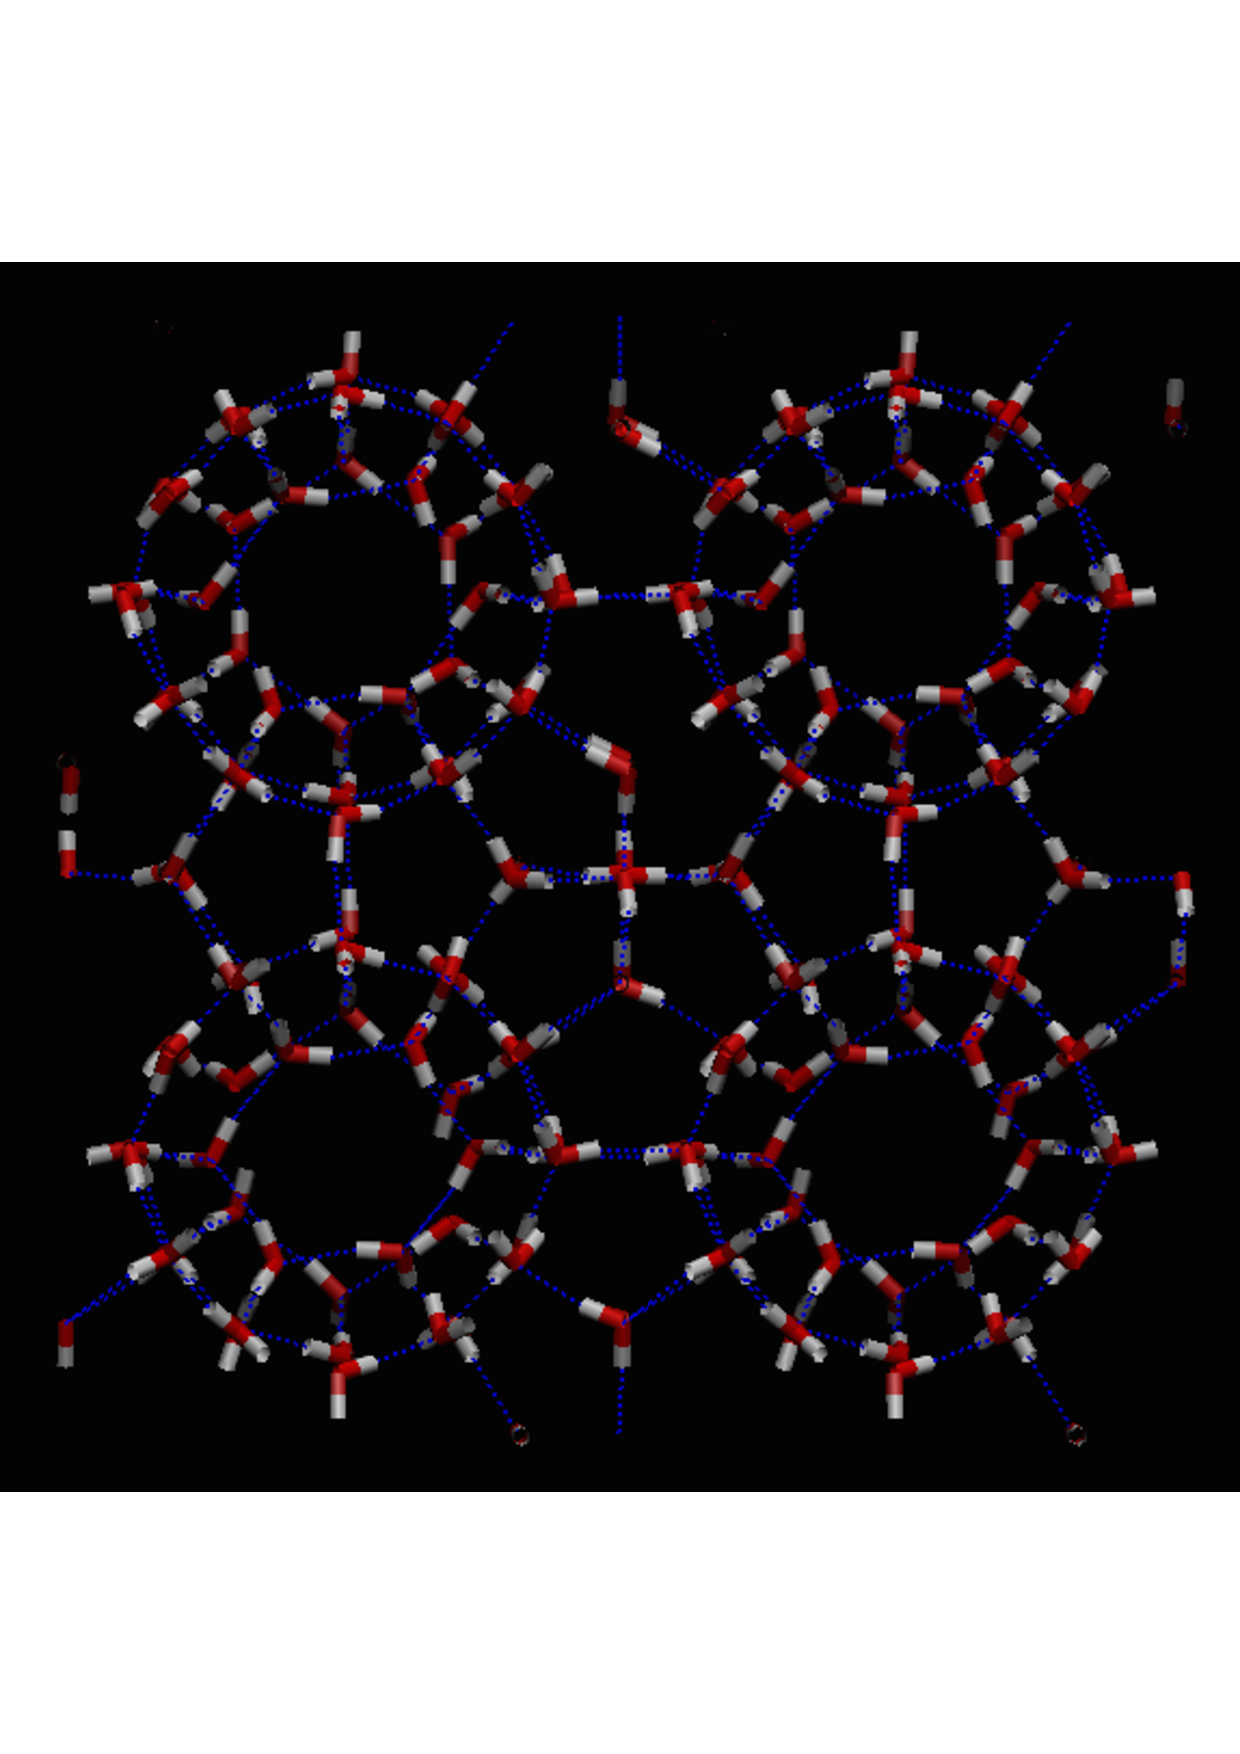
\includegraphics[width=\textwidth]{../snapshots/first_stable_hydrate.pdf}
\caption{Methane hydrate at low temperature. Rendered with VMD}
\label{fig:part2:first_hydrate}
\end{figure}

\section{Three-phase equilibrium line for methane hydrate}
Three-phase equilibrium simulations have been performed to check whether the model system is in the same ballpark as systems from the literature. Simulations have been performed on a system similar to the one in \cite{Conde2010}.

\section{Nucleation of methane hydrates?}
Nucleation of methane hydrates in a solution of water and methane is a rare event, and microsectond-simulations are required. 
